
% This LaTeX was auto-generated from MATLAB code.
% To make changes, update the MATLAB code and republish this document.
\documentclass[a4paper,fleqn,12pt]{article}

\usepackage[utf8]{inputenc}
\usepackage[bulgarian]{babel}
\usepackage{graphicx}
\usepackage{color}

\sloppy
\definecolor{lightgray}{gray}{0.5}
\setlength{\parindent}{0pt}

\begin{document}

    
\begin{verbatim}
function firstTask
% Дефиниране на началните условия
y0 = [0; -1/6];
x0 = 0;
% Дефиниране на стъпката и броя на стъпките
h = 0.1;
n = 100;
% Използване на RK4 функцията
[x, y] = RK4(@system, x0, y0, h, n);
% Графика на резултатите
plot(x,y(1,:),x,y(2,:));
title('Решение на системата по Рунге-Кута');
legend('y1', 'y2', 'Location', 'southwest', 'Orientation', 'vertical');
xlabel('x');
end

function [x, y] = RK4(f, x0, y0, h, n)
% f - функция, която връща дясната част на системата
% x0 - начална точка за решението
% y0 - началните условия
% h - стъпка на метода
% n - брой стъпки

x = x0 + (0:n-1)*h;  % Изчисляваме x стойностите
y = zeros(length(y0), n);  % Създаваме матрица за y
y(:,1) = y0;  % Запазваме началните условия в първата колона на y
for i = 1:n-1
    k1 = f(x(i), y(:,i));
    k2 = f(x(i)+0.5*h, y(:,i)+0.5*h*k1);
    k3 = f(x(i)+0.5*h, y(:,i)+0.5*h*k2);
    k4 = f(x(i)+h, y(:,i)+h*k3);
    y(:,i+1) = y(:,i) + h*(k1+2*k2+2*k3+k4)/6;  % Изчисляваме y_i+1
end
end

function dydx = system(x, y)
a = 0.05;
dydx = [y(2); -a*y(2) - x^2*y(1)];
end
\end{verbatim}

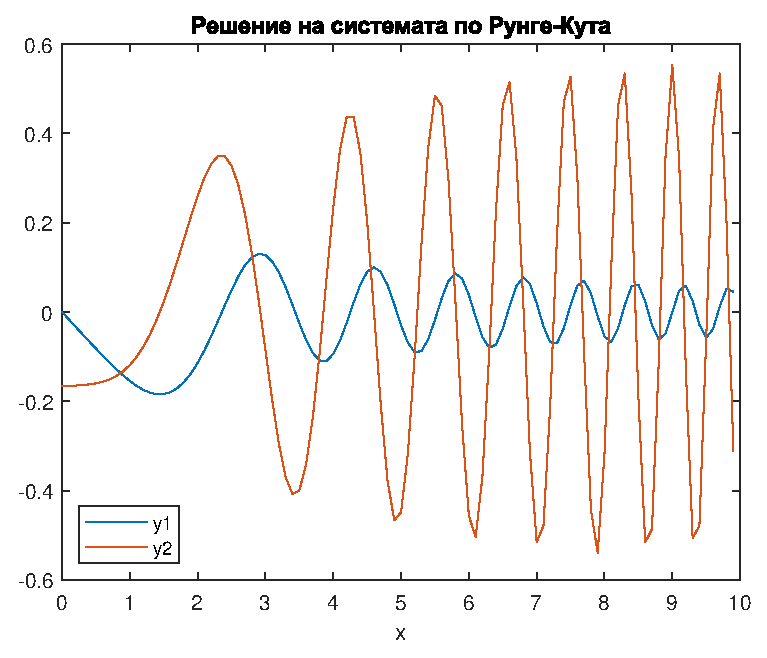
\includegraphics [width=4in]{firstTask_01.eps}



\end{document}

